\PassOptionsToPackage{dvipsnames}{xcolor}  % avoid options class with metropolis theme
\documentclass[aspectratio=169]{beamer} 

\usepackage{hayesmacros}

% \usepackage[dvips]{xcolor}
\usetheme[numbering=none]{metropolis}
\setsansfont{Fira Sans}  % be sure to compile with XeLaTeX
% \setmonofont{Fira Mono}  % be sure to compile with XeLaTeX

\usepackage{natbib}
\usepackage{nicematrix}
\usepackage{fontawesome5}

\newtheorem{proposition}{Proposition}
\newtheorem{assumption}{Assumption}
\theoremstyle{remark}
\newtheorem*{remark}{Remark}

\setbeamercolor{background canvas}{bg=white}
\setbeamercolor{normal text}{fg=black}
\setbeamercolor{frametitle}{bg=black, fg=white}

\hypersetup{colorlinks,allcolors=black}


\title{Asymptotic identifiability of peer effects in the linear-in-means model}
\date{2024-04-04}
\author{Alex Hayes | PhD Defense}
\institute{Department of Statistics, University of Wisconsin-Madison}

\begin{document}

\maketitle

% \begin{frame}
%     \begin{itemize}
%         \item Keith Levin
%         \item Karl Rohe
%         \item Hyunseung Kang
%         \item Felix Elwert
%         \item Sameer Deshpande
%     \end{itemize}
% \end{frame}

\begin{frame}{Social scientists study social networks}
    \begin{columns}
        \column{0.4\textwidth}
        \centering
        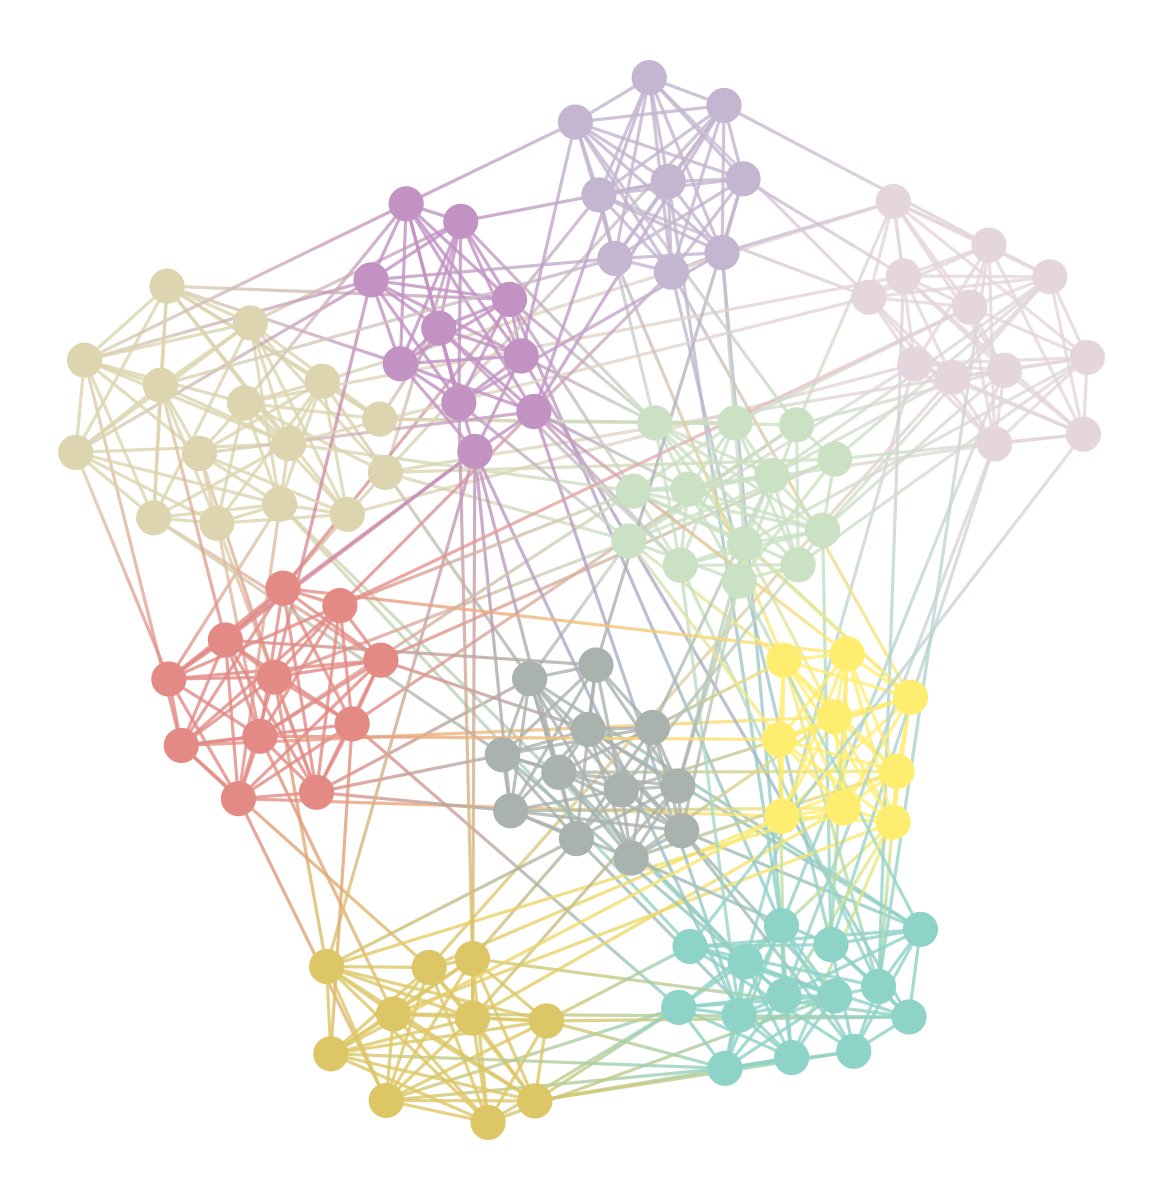
\includegraphics[width=\textwidth]{./assortative.png}
        \column{0.6\textwidth}
        \onslide<1->{
            % \underline{Social networks}
            % for nodes $i, j \in \set{1, \dots, n}$
            \vspace{4mm} \\
            \begin{table}[]
                \begin{tabular}{llcl}
                    \onslide<1->{%
                    Nodes           & (people)      & $i$      & $\in \set{1, \dots, n}$  \\
                    }
                    \onslide<2->{%
                                    &               &          &                          \\
                    Edge $i \sim j$ & (friends?)    & $A_{ij}$ & $\in \{0, 1\}$           \\
                    Degree          & (num friends) & $d_i$    & $\in \set{0, 1, 2, ...}$ \\
                    }
                    \onslide<3->{%
                                    &               &          &                          \\
                    Outcome         & (sick?)       & $Y_i$    & $\in \R$                 \\
                    Treatment       & (vaccinated?) & $T_i$    & $\in \R$                 \\
                    }
                \end{tabular}
            \end{table}
        }
    \end{columns}
\end{frame}


\begin{frame}{Peer effects quantify social influence}
    \begin{columns}
        \column{0.4\textwidth}
        \centering
        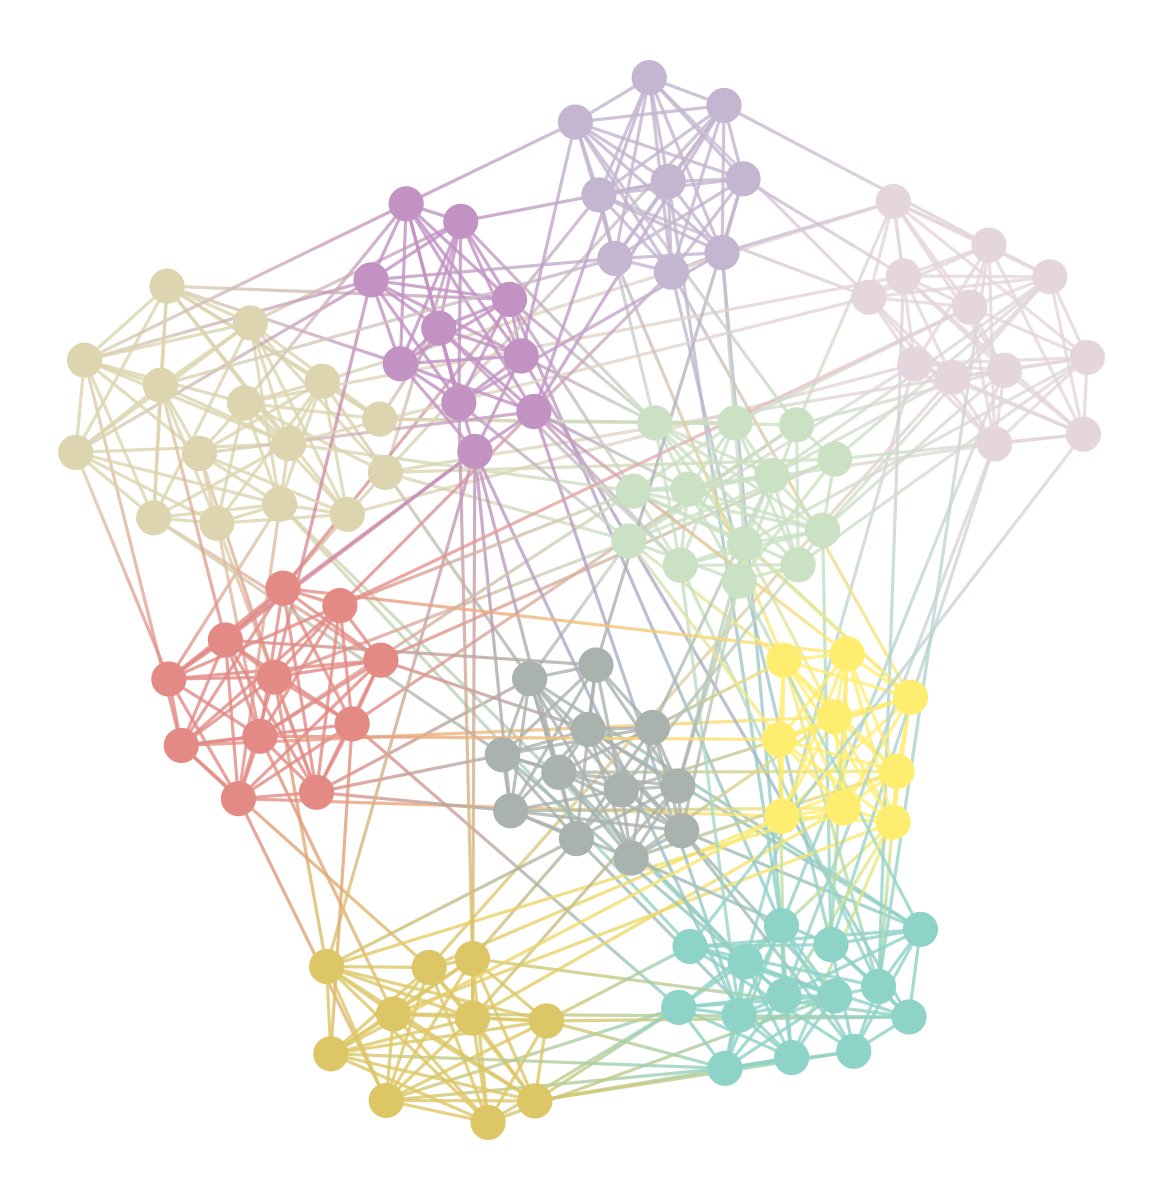
\includegraphics[width=\textwidth]{./assortative.png}
        \column{0.6\textwidth}
        % \begin{center} Peer effects  \\ \end{center}
        \vspace{4mm} \\
        \onslide<1->{
            \underline{Contagion}: if my friends get sick, I am more likely to get sick \\   
            \vspace{4mm}
            \underline{Direct effect}: if I get vaccinated, I am less likely to get sick \\
            \vspace{4mm}
            \underline{Interference}: if my friends get vaccinated, I am less likely to get sick \\
            \vspace{7mm}
        }
        \onslide<2->{
            \footnotesize * Can be defined counterfactually, but we define peer effects without counterfactuals in this talk.
        }
    \end{columns}
\end{frame}

\begin{frame}{Social scientists study peer effects using the \underline{linear-in-means} model}
    \footnotesize
    \begin{table}[]
        \begin{tabular}{llcl@{\hspace{4em}}lcl}
            Outcome         & (sick?)       & $Y_i$    & $\in \{0, 1\}$             & Base rate     & $\alpha$ & $\in \R$      \\
            Treatment       & (vaccinated?) & $T_i$    & $\in \{0, 1\}$             & Contagion     & $\beta$  & $\in (-1, 1)$ \\
            Edge $i \sim j$ & (friends?)    & $A_{ij}$ & $\in \{0, 1\}$             & Direct effect & $\gamma$ & $\in \R$      \\
            Node degree     & (num friends) & $d_i$    & $\in \set{0, 1, 2, \dots}$ & Interference  & $\delta$ & $\in \R$      \\
        \end{tabular}
    \end{table}
    \Large
    \vspace{4mm}
    \begin{equation*}
        \onslide<1->{
            Y_i =
            \alpha
        }
        \onslide<2->{
            + \beta \underbrace{\frac{1}{d_i} \sum_{j \, : \, A_{ij} = 1} Y_j}_{\substack{\text{fraction} \\ \text{sick} \\ \text{friends}}}
        }
        \onslide<3->{
            + \gamma T_i
        }
        \onslide<4->{
            + \delta \underbrace{\frac{1}{d_i} \sum_{j \, : \, A_{ij} = 1} T_j}_{\substack{\text{fraction} \\ \text{vaccinated} \\ \text{friends}}}
        }
        \onslide<5-> {
            + \underbrace{\varepsilon_i}_\text{error}
        }
    \end{equation*}
    % \begin{equation*}
    %     Y_i =
    %     \alpha +
    %     \beta
    %     \underbrace{\frac{1}{d_i} \sum_{j \, : \, A_{ij} = 1} Y_j}_{\substack{\text{fraction} \\ \text{sick} \\ \text{friends}}} + 
    %     \gamma
    %     T_i + 
    %     \delta
    %     \underbrace{\frac{1}{d_i} \sum_{j \, : \, A_{ij} = 1} T_j}_{\substack{\text{fraction} \\ \text{vaccinated} \\ \text{friends}}} +
    %     \underbrace{\varepsilon_i}_\text{error}
    % \end{equation*}
    
\end{frame}

\begin{frame}{Social scientists study peer effects using the \underline{linear-in-means} model}
    \onslide<1->{
        \footnotesize
        \begin{columns}
            \begin{column}{0.51\textwidth}
                $[GY]_i = $ ``fraction of $i$'s friends who are sick'' \\
                $[GT]_i = $ ``fraction of $i$'s friends who are vaccinated'' \\
            \end{column}
            \begin{column}{0.5\textwidth}
                $D = \diag(d_1, \dots, d_n) \in \R^{n \times n}$ and $G = D^{-1} A \in \R^{n \times n}$ \\
                $G$ computes averages of a value among friends \\
            \end{column}
        \end{columns}
        \normalsize
    }
    \onslide<2->{
        \begin{equation*}
            \begin{bmatrix}
                Y_1    \\
                Y_2    \\
                \vdots \\
                Y_n
            \end{bmatrix}
            =
            \begin{bNiceMatrix}[first-row,first-col]
                 &        &        &        &        \\
                 & 1      & [GY]_1 & T_1    & [GT]_1 \\
                 & 1      & [GY]_2 & T_2    & [GT]_2 \\
                 & \vdots & \vdots & \vdots & \vdots \\
                 & 1      & [GY]_n & T_n    & [GT]_n \\
            \end{bNiceMatrix}
            \begin{bmatrix}
                \alpha \\
                \beta  \\
                \gamma \\
                \delta
            \end{bmatrix}
            +
            \begin{bmatrix}
                \varepsilon_1 \\
                \varepsilon_2 \\
                \vdots        \\
                \varepsilon_n
            \end{bmatrix}
        \end{equation*} \\
    }
    \vspace{4mm}
    \onslide<3-> {
        \vspace{4mm}
        \centering
        $\E[T, GT]{\varepsilon} = 0$ but $\mathrm{Cov}\paren*{GY, \varepsilon} \neq 0$ because $Y$ is on both sides of the equation
    }
\end{frame}

\begin{frame}{Identification in the linear-in-means model is subtle}
    \begin{proposition}[\citealt{bramoulle2009}]
        Suppose there are no isolated nodes in the network. Then $(\alpha, \beta, \gamma, \delta)$ are identified if and only if $1_n, \E[T, GT]{GY}, T$ and $GT$ are linearly independent.
    \end{proposition}
    \begin{equation*}
        \begin{bmatrix}
            Y_1    \\
            Y_2    \\
            \vdots \\
            Y_n
        \end{bmatrix}
        =
        \begin{bNiceMatrix}[first-row,first-col]
             &        &        &        &        \\
             & 1      & [GY]_1 & T_1    & [GT]_1 \\
             & 1      & [GY]_2 & T_2    & [GT]_2 \\
             & \vdots & \vdots & \vdots & \vdots \\
             & 1      & [GY]_n & T_n    & [GT]_n \\
        \end{bNiceMatrix}
        \begin{bmatrix}
            \alpha \\
            \beta  \\
            \gamma \\
            \delta
        \end{bmatrix}
        +
        \begin{bmatrix}
            \varepsilon_1 \\
            \varepsilon_2 \\
            \vdots        \\
            \varepsilon_n
        \end{bmatrix}
    \end{equation*} \\
    \vspace{4mm}
    Very similar to the usual requirement in linear models that the columns of the design matrix are linearly independent
\end{frame}

\begin{frame}{Identification depends heavily on network structure}
    \vspace{5mm}
    \begin{figure}
        \centering
        
\includegraphics[width=0.9\textwidth]{./manski1993.png}
    \end{figure}
\end{frame}

\begin{frame}{Too much structure in the network can cause collinearity}
    \centering
    \vspace{4mm}
    \tikzset{every loop/.style={}}
    \begin{columns}
        \begin{column}{0.5\textwidth}
            \onslide<1->{
                \begin{figure}
                    \centering
                    \begin{tikzpicture}
                        \node[shape=circle,fill=MidnightBlue,label=above left:{$T_1 = 1$}] (A) at (0,1) {};
                        \node[shape=circle,fill=MidnightBlue,label=below left:{$T_2 = 0$}] (B) at (1,0) {};
                        \node[shape=circle,fill=MidnightBlue,label=above right:{$T_3 = 1$}] (C) at (1.5,1.5) {};
                        \node[shape=circle,fill=MidnightBlue,label=above right:{$T_4 = 1$}] (D) at (2.75,0.5) {};
                        
                        \path (A) edge [loop above] node {} (A);
                        \path (B) edge [loop below] node {} (B);
                        \path (C) edge [loop above] node {} (C);
                        \path (D) edge [loop above] node {} (D);
                        
                        \draw (A) -- (B);
                        \draw (A) -- (C);
                        \draw (A) -- (D);
                        \draw (B) -- (C);
                        \draw (B) -- (D);
                        \draw (C) -- (D);
                    \end{tikzpicture}
                \end{figure}
            }
        \end{column}
        \begin{column}{0.5\textwidth}
            \onslide<2->{
                \begin{figure}
                    \centering
                    \begin{tikzpicture}
                        \node[shape=circle,fill=MidnightBlue,label=above left:{$[GT]_1 = 3/4$}] (A) at (0,1) {};
                        \node[shape=circle,fill=MidnightBlue,label=below left:{$[GT]_2 = 3/4$}] (B) at (1,0) {};
                        \node[shape=circle,fill=MidnightBlue,label=above right:{$[GT]_3 = 3/4$}] (C) at (1.5,1.5) {};
                        \node[shape=circle,fill=MidnightBlue,label=above right:{$[GT]_4 = 3/4$}] (D) at (2.75,0.5) {};
                        
                        \path (A) edge [loop above] node {} (A);
                        \path (B) edge [loop below] node {} (B);
                        \path (C) edge [loop above] node {} (C);
                        \path (D) edge [loop above] node {} (D);
                        
                        \draw (A) -- (B);
                        \draw (A) -- (C);
                        \draw (A) -- (D);
                        \draw (B) -- (C);
                        \draw (B) -- (D);
                        \draw (C) -- (D);
                    \end{tikzpicture}
                \end{figure}
            }
        \end{column}
    \end{columns}
\end{frame}

\begin{frame}{Too much structure in the network can cause collinearity}
    \centering
    \begin{equation*}
        \begin{bmatrix}
            Y_1 \\
            Y_2 \\
            Y_3 \\
            Y_4
        \end{bmatrix}
        =
        \begin{bNiceMatrix}[first-row,first-col]
             &                         &      &   &                           \\
             & \textcolor{BrickRed}{1} & GY_1 & 1 & \textcolor{BrickRed}{3/4} \\
             & \textcolor{BrickRed}{1} & GY_2 & 0 & \textcolor{BrickRed}{3/4} \\
             & \textcolor{BrickRed}{1} & GY_3 & 1 & \textcolor{BrickRed}{3/4} \\
             & \textcolor{BrickRed}{1} & GY_4 & 1 & \textcolor{BrickRed}{3/4} \\
        \end{bNiceMatrix}
        \begin{bmatrix}
            \textcolor{BrickRed}{\alpha} \\
            \beta                        \\
            \gamma                       \\
            \textcolor{BrickRed}{\delta}
        \end{bmatrix}
        +
        \begin{bmatrix}
            \varepsilon_1 \\
            \varepsilon_2 \\
            \varepsilon_3 \\
            \varepsilon_4
        \end{bmatrix}
    \end{equation*}
    
    Can't distinguish base rate $\textcolor{BrickRed}{\alpha}$ from interference $\textcolor{BrickRed}{\delta}$
\end{frame}

% \begin{frame}{Identification}

%     Define the degree matrix $D = \diag(d_1, d_2, \dots, d_n)$, where $d_i = \sum_j A_{ij}$. Let $G = D^{-1} A$ be the row-normalized adjacency matrix. Then
%     \begin{equation*} \label{eq:lim-mv}
%         Y = \alpha 1_n + \beta G Y + T \gamma + G T \delta + \varepsilon.
%     \end{equation*}

%     \begin{definition}
%         We say that $(\alpha, \beta, \gamma, \delta)$ are \underline{identified} when the columns of the design matrix 
%         \begin{equation*}
%             \label{eq:design}
%             W_n = \begin{bmatrix} 1_n & GY & T & GT \end{bmatrix}.
%         \end{equation*}
%         are linearly independent. Otherwise, we say that $(\alpha, \beta, \gamma, \delta)$ are \underline{unidentified}.
%     \end{definition}

%     We assume that $\mathbb E \left[\varepsilon | W_n \right] = 0$.
% \end{frame}

\begin{frame}{Typical networks don't exhibit problematic structure}
    \begin{figure}
        \centering
        
\includegraphics[width=\textwidth]{./bramoulle2009.png}
    \end{figure}
\end{frame}

\begin{frame}{Peer effects are identified if there is 1+ open triangle in the network}
    \centering
    \cite{bramoulle2009}: ``intransitivity'' identifies peer effects
    \vspace{8mm}
    \begin{columns}
        \begin{column}{0.4\textwidth}
            \centering
            \begin{tikzpicture}
                \node[shape=circle,fill=MidnightBlue,label=above left:A] (A) at (0,1) {};
                \node[shape=circle,fill=MidnightBlue,label=below left:B] (B) at (1,0) {};
                \node[shape=circle,fill=MidnightBlue,label=above right:C] (C) at (1.5,1.5) {};
                \node[shape=circle,fill=MidnightBlue,label=above right:D] (D) at (2.75,0.5) {};
                \draw (A) -- (B);
                \draw (A) -- (C);
                \draw (B) -- (C);
                \draw (C) -- (D);
            \end{tikzpicture}
        \end{column}
        \begin{column}{0.6\textwidth}
            \centering
            % \underline{i.e., 1+ open triangle identifies peer effects} \\
            % \vspace{4mm}
            Closed: \textcolor{BrickRed}{$A \leftrightarrow B \leftrightarrow C \leftrightarrow A$} \\
            Open: $B \leftrightarrow C \leftrightarrow D \nleftrightarrow B$
        \end{column}
    \end{columns}
\end{frame}

\begin{frame}{We ran an experiment on a model with many open triangles}
    \vspace{3mm}
    \centering
    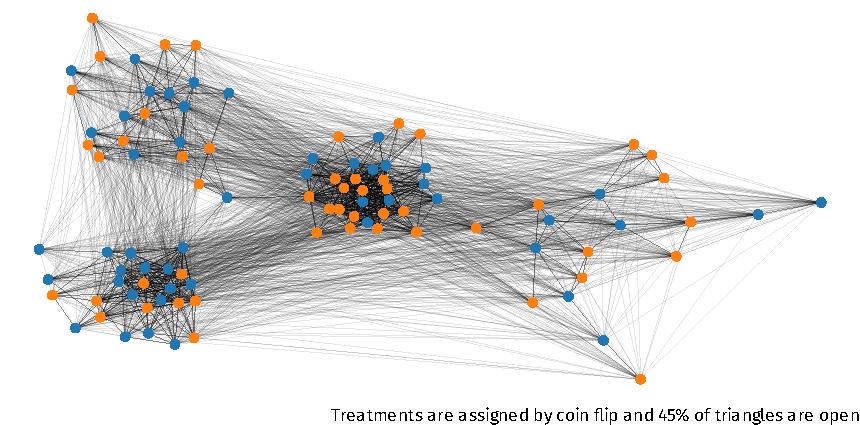
\includegraphics{./figures/simulations/defense-backbone.pdf}
\end{frame}

\begin{frame}{In the experiment, we couldn't recover the regression coefficients}
    \vspace{3mm}
    \centering
    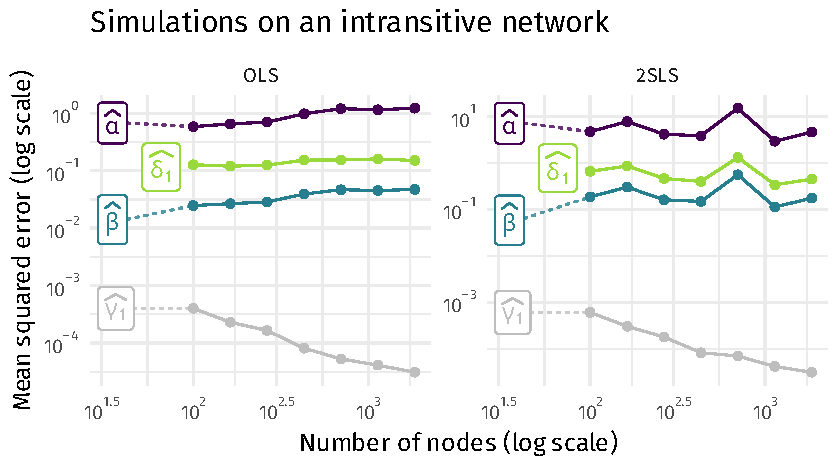
\includegraphics{./figures/simulations/defense-mse.pdf}
\end{frame}

\begin{frame}{The interference column converges to a constant in large samples}
    \centering
    \onslide<3->{
        When the network grows ($n \to \infty$),
    }
    \onslide<4->{
        if everyone makes more friends ($d_i \to \infty$)
    }
    \Large
    \vspace{6mm}
    \begin{equation*}
        \onslide<3->{
            \lim_{n \to \infty}
        }
        \onslide<1->{
            \underbrace{[GT]_i}_{\substack{\text{fraction} \\ \text{vaccinated} \\ \text{friends}}}
        }
        \onslide<2->{=}
        \onslide<3->{
            \lim_{n \to \infty}
        }
        \onslide<2->{
            \underbrace{
                \frac{1}{d_i} \sum_{j \, : \, A_{ij} = 1} T_j
            }_{\substack{\text{average of $d_i$}           \\ \text{i.i.d. coin flips}}}
        }
        \onslide<4->{
            = \frac 12   
        }
    \end{equation*} \\
    \normalsize
    \vspace{6mm}
    \onslide<5->{
        \underline{For every single node $i = 1, ..., n$}
    }
\end{frame}

\begin{frame}{Base rates and interence are indistinguishable in large samples}
    \centering
    \begin{equation*}
        \begin{bmatrix}
            Y_1    \\
            Y_2    \\
            \vdots \\
            Y_n
        \end{bmatrix}
        =
        \underbrace{
            \begin{bNiceMatrix}[first-row,first-col]
                 & 1_n                     & GY     & T      & GT                        \\
                 & \textcolor{BrickRed}{1} & GY_1   & 1      & \textcolor{BrickRed}{1/2} \\
                 & \textcolor{BrickRed}{1} & GY_2   & 0      & \textcolor{BrickRed}{1/2} \\
                 & \vdots                  & \vdots & \vdots & \vdots                    \\
                 & \textcolor{BrickRed}{1} & GY_n   & 1      & \textcolor{BrickRed}{1/2}
            \end{bNiceMatrix}
        }_\text{as $n \to \infty$}
        \begin{bmatrix}
            \textcolor{BrickRed}{\alpha} \\
            \beta                        \\
            \gamma                       \\
            \textcolor{BrickRed}{\delta}
        \end{bmatrix}
        +
        \begin{bmatrix}
            \varepsilon_1 \\
            \varepsilon_2 \\
            \vdots        \\
            \varepsilon_n
        \end{bmatrix}
    \end{equation*} \\
    \vspace{8mm}
    \underline{Can't distinguish between base rate $\textcolor{BrickRed}{\alpha}$ and interference $\textcolor{BrickRed}{\delta}$}
\end{frame}

\begin{frame}{Base rates, interference and contagion are indistinguishable in large samples}
    
    \begin{equation*}
        \begin{bmatrix}
            Y_1    \\
            Y_2    \\
            \vdots \\
            Y_n
        \end{bmatrix}
        =
        \underbrace{
            \begin{bNiceMatrix}[first-row,first-col]
                 & 1_n                     & GY                         & T      & GT                        \\
                 & \textcolor{BrickRed}{1} & \textcolor{BrickRed}{\eta} & 1      & \textcolor{BrickRed}{1/2} \\
                 & \textcolor{BrickRed}{1} & \textcolor{BrickRed}{\eta} & 0      & \textcolor{BrickRed}{1/2} \\
                 & \vdots                  & \vdots                     & \vdots & \vdots                    \\
                 & \textcolor{BrickRed}{1} & \textcolor{BrickRed}{\eta} & 1      & \textcolor{BrickRed}{1/2}
            \end{bNiceMatrix}
        }_\text{as $n \to \infty$}
        \begin{bmatrix}
            \textcolor{BrickRed}{\alpha} \\
            \textcolor{BrickRed}{\beta}  \\
            \gamma                       \\
            \textcolor{BrickRed}{\delta}
        \end{bmatrix}
        +
        \begin{bmatrix}
            \varepsilon_1 \\
            \varepsilon_2 \\
            \vdots        \\
            \varepsilon_n
        \end{bmatrix}
    \end{equation*} \\
    \vspace{6mm}
    \begin{center}
        \underline{Can't distinguish between base rate $\textcolor{BrickRed}{\alpha}$, interference $\textcolor{BrickRed}{\delta}$ and contagion $\textcolor{BrickRed}{\beta}$} \\
    \end{center}
\end{frame}

\begin{frame}{Outcomes are generated by diffusing the treatment over the network}
    \begin{align*}
        \onslide<1-> {
        Y             & = \alpha 1_n + \beta G Y + \gamma T + \delta G T + \varepsilon                                         \\
        }
        \onslide<2-> {
        Y - \beta G Y & = \alpha 1_n  + \gamma T + \delta G T + \varepsilon                                                    \\
        }
        \onslide<3->{
        Y             & = \paren*{I - \beta G}^{-1} \paren*{\alpha 1_n + \gamma T + \delta G T + \varepsilon}                  \\
        }
        \onslide<4->{
                      & \overset{*}{=} \sum_{k=0}^\infty \beta^k G^k \paren*{\alpha 1_n + \gamma T + \delta G T + \varepsilon} \\
        }
        \onslide<5->{
                      & = \frac{\alpha}{1 - \beta} 1_n +
        \gamma T +
        \underbrace{(\gamma \beta + \delta) \sum_{k=0}^\infty \beta^k G^{k+1} T}_{\substack{\text{repeated}                    \\ \text{averages} \\ \text{of $T$}}} +
        \underbrace{\sum_{k=0}^\infty \beta^k G^k \varepsilon}_{\substack{\text{repeated}                                      \\ \text{averages} \\ \text{of $\varepsilon$}}}
        }
    \end{align*} \\
    \vspace{2mm}
    \footnotesize
    \onslide<4->{
        $^*$ using the fact that $\paren*{I - \beta G}^{-1} = \sum_{k=0}^\infty \beta^k G^k$ when $\abs*{\beta} < 1$
    }
    
\end{frame}

\begin{frame}{The contagion column converges to a constant in large samples}
    \begin{align*}
        GY = 
        \frac{\alpha}{1 - \beta} 1_n + 
        \underbrace{\gamma G T}_{\substack{\text{neighborhood}                                              \\ \text{average } \to \gamma / 2}} + 
        \underbrace{(\gamma \beta + \delta) \sum_{k=0}^\infty \beta^k G^{k+2} T}_{\substack{\text{repeated} \\ \text{averages} \\ \text{of $T$ *}}} +
        \underbrace{\sum_{k=0}^\infty \beta^k G^{k+1} \varepsilon}_{\substack{\text{repeated}               \\ \text{averages} \\ \text{of $\varepsilon$ } \to \, 0}}
    \end{align*} \\
    \vspace{4mm}
    Each term converges to a constant, call the sum of these constants $\eta$. Then
    \begin{align*}
        GY            & \to \eta   \\
        \E[T, GT]{GY} & \to \eta 
    \end{align*} \\
    \vspace{4mm}
    \footnotesize
    * If $c \in R$ and $GT = c 1_n$, then $G^2 T = G (GT) = G (c 1_n) = c 1_n$. i.e., $G^2 T = GT$
\end{frame}

\begin{frame}{Base rates, interference and contagion are indistinguishable in large samples}
    
    \begin{equation*}
        \begin{bmatrix}
            Y_1    \\
            Y_2    \\
            \vdots \\
            Y_n
        \end{bmatrix}
        =
        \underbrace{
            \begin{bNiceMatrix}[first-row,first-col]
                 & 1_n                     & GY                         & T      & GT                        \\
                 & \textcolor{BrickRed}{1} & \textcolor{BrickRed}{\eta} & 1      & \textcolor{BrickRed}{1/2} \\
                 & \textcolor{BrickRed}{1} & \textcolor{BrickRed}{\eta} & 0      & \textcolor{BrickRed}{1/2} \\
                 & \vdots                  & \vdots                     & \vdots & \vdots                    \\
                 & \textcolor{BrickRed}{1} & \textcolor{BrickRed}{\eta} & 1      & \textcolor{BrickRed}{1/2}
            \end{bNiceMatrix}
        }_\text{as $n \to \infty$}
        \begin{bmatrix}
            \textcolor{BrickRed}{\alpha} \\
            \textcolor{BrickRed}{\beta}  \\
            \gamma                       \\
            \textcolor{BrickRed}{\delta}
        \end{bmatrix}
        +
        \begin{bmatrix}
            \varepsilon_1 \\
            \varepsilon_2 \\
            \vdots        \\
            \varepsilon_n
        \end{bmatrix}
    \end{equation*} \\
    \vspace{6mm}
    \begin{center}
        \underline{Can't distinguish between base rate $\textcolor{BrickRed}{\alpha}$, interference $\textcolor{BrickRed}{\delta}$ and contagion $\textcolor{BrickRed}{\beta}$} \\
    \end{center}
    \vspace{6mm}
    \footnotesize
    * Recall that identifiability depends on $\E[T, GT]{GY}$ but last slide also implies $\E[T, GT]{GY} \to \eta$
\end{frame}

\begin{frame}{We call these indistinguishable parameters asymptotically unidentified}
    \begin{definition}
        We say that $(\alpha, \beta, \gamma, \delta)$ are \underline{asymptotically identified} when the design matrix $W_n$ converges to a limit object $W$ in the sense that
        \begin{equation*}
            \max_{ij} \abs*{
            \begin{bmatrix} 1_n & GY & T & GT \end{bmatrix}_{ij} - W_{ij}
            } = o(1)
        \end{equation*}
        and the columns of $W$ are linearly independent. If the columns of $W$ are linearly dependent, we say that $(\alpha, \beta, \gamma, \delta)$ are \underline{asymptotically unidentified}.
    \end{definition}
\end{frame}

\begin{frame}{Peer effects are asymptotically unidentified under very general circumstances}
    \begin{assumption}
        \begin{enumerate}
            \item $T_1,T_2,\dots,T_n$ are independent with shared mean $\zeta \in \R$, and $T$ is independent of $A$.
            \item $\{ T_i - \zeta : i \in [n] \}$ are independent $(\nu,b)$-subgamma random variables.
            \item $\varepsilon_1, \varepsilon_2, \dots, \varepsilon_n$ are independent subgamma random variables with parameters not depending on $n$.
            \item The minimum degree grows strictly faster than $\log n$, such that
                  \begin{equation*}
                      \lim_{n \to \infty} \frac{\min_{i \in [n]} d_i}{\log n} = \infty
                  \end{equation*}
        \end{enumerate}
    \end{assumption}
\end{frame}

\begin{frame}{The interference and contagion columns converge uniformly to constants}
    
    \begin{lemma}
        Under the previous assumptions,
        \begin{equation*}
            \max_{i \in [n]} \Big\| [GT]_i - \zeta \Big\|
            = o(1) ~ \text{ almost surely }
        \end{equation*}
        and there exists $\eta = \eta(\zeta, \alpha, \beta, \gamma, \delta) \in \R$ such that
        \begin{equation*}
            \max_{i \in [n]} \Big\| [GY]_i - \eta \Big\|
            = o(1) ~ \text{ almost surely.}
        \end{equation*}
    \end{lemma}
    
    \begin{quote}
        \footnotesize Read: ``The fraction of $i$'s friends who are vaccinated $[GT]_i$ and fraction of $i$'s friends who are sick $[GY]_i$ converge to constants $\zeta$ and $\eta$, respectively, for all nodes $i = 1, ..., n$.''
    \end{quote}
    
    \begin{theorem}
        $\textcolor{BrickRed}{\alpha}, \textcolor{BrickRed}{\beta}$ and $\textcolor{BrickRed}{\delta}$ are asymptotically unidentified.
    \end{theorem}
\end{frame}

\begin{frame}{\textcolor{BrickRed}{Asymptotically unidentified} coefficients become collinear in finite samples}
    \vspace{3mm}
    \centering
    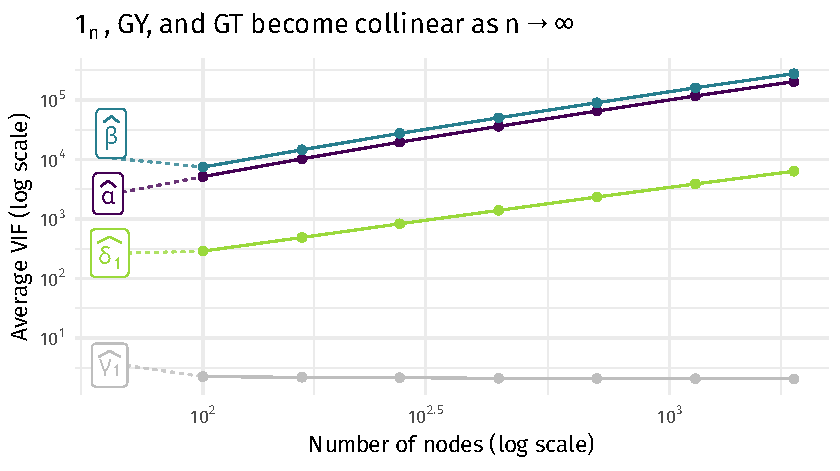
\includegraphics{./figures/simulations/defense-vif.pdf}
\end{frame}

\begin{frame}{\textcolor{BrickRed}{Asymptotically unidentified} coefficients cannot be estimated}
    \vspace{3mm}
    \centering
    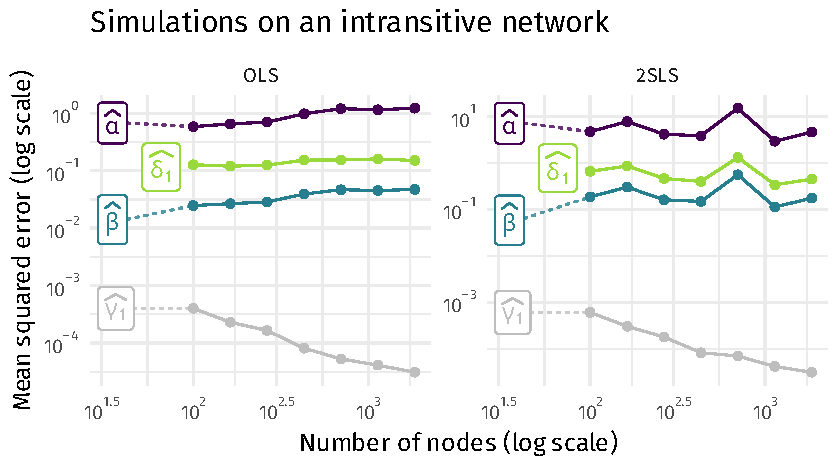
\includegraphics{./figures/simulations/defense-mse.pdf}
\end{frame}

\begin{frame}{Our theory does not apply to sparse networks or fixed covariates}
    \underline{Isolated nodes}: If all the connected components that are not singletons satisfy previous assumptions, can recover $\alpha$ but $\beta$ and $\delta$ are still aliased. \\
    \vspace{5mm}
    \underline{Sparse networks}: we don't know exactly when the issue kicks in and if sparse networks are in trouble or not \\
    \vspace{5mm}
    \underline{Non-random treatment $T$}: theorem doesn't apply
\end{frame}

\begin{frame}{Our theory does apply to weighted and directed networks}
    \underline{Weighted networks}: If $A \in \R^{n \times n}$ is a weighted network with $(\nu, b)$-subgamma edges $A_{ij}$, we require that
    \begin{equation*}
        \max_{i \in [n]} \frac{1}{d_i^2} \sum_{j=1}^n A_{ij}^2
        = o\left( \frac{ 1 }{ \nu \log^2 n } \right)
        ~\text{ and }~
        \max_{j \in [n]} \frac{ A_{ij} }{ d_i }
        = o\left( \frac{ 1 }{ b \log n } \right).
    \end{equation*} \\
    \vspace{5mm}
    \underline{Directed networks}: extension possible, but slightly more involved
\end{frame}

\begin{frame}{What happens when treatment depends on position in network?}
    \centering
    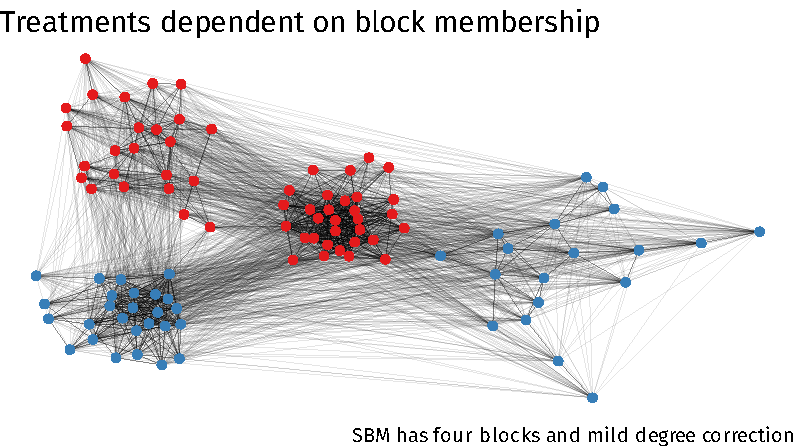
\includegraphics{./figures/simulations/defense-backbone-dependent.pdf}
\end{frame}

\begin{frame}{Dependence between treatment and network might recover identifiability}
    \Large
    \begin{align*}
        \underbrace{[GT]_i}_{\substack{\text{fraction} \\ \text{vaccinated} \\ \text{friends}}}
        = \underbrace{
            \frac{1}{d_i} \sum_{j \, : \, A_{ij} = 1} T_j
        }_{\substack{\text{average of dependent treatments}}}
    \end{align*} \\
    \normalsize
    \centering
    \vspace{8mm}
    $GT$ might not coverge, or might converge to non-constant value
\end{frame}

\begin{frame}{We investigate identification when treatments depend on network structure}
    \begin{columns}
        \column{0.45\textwidth}
        \centering
        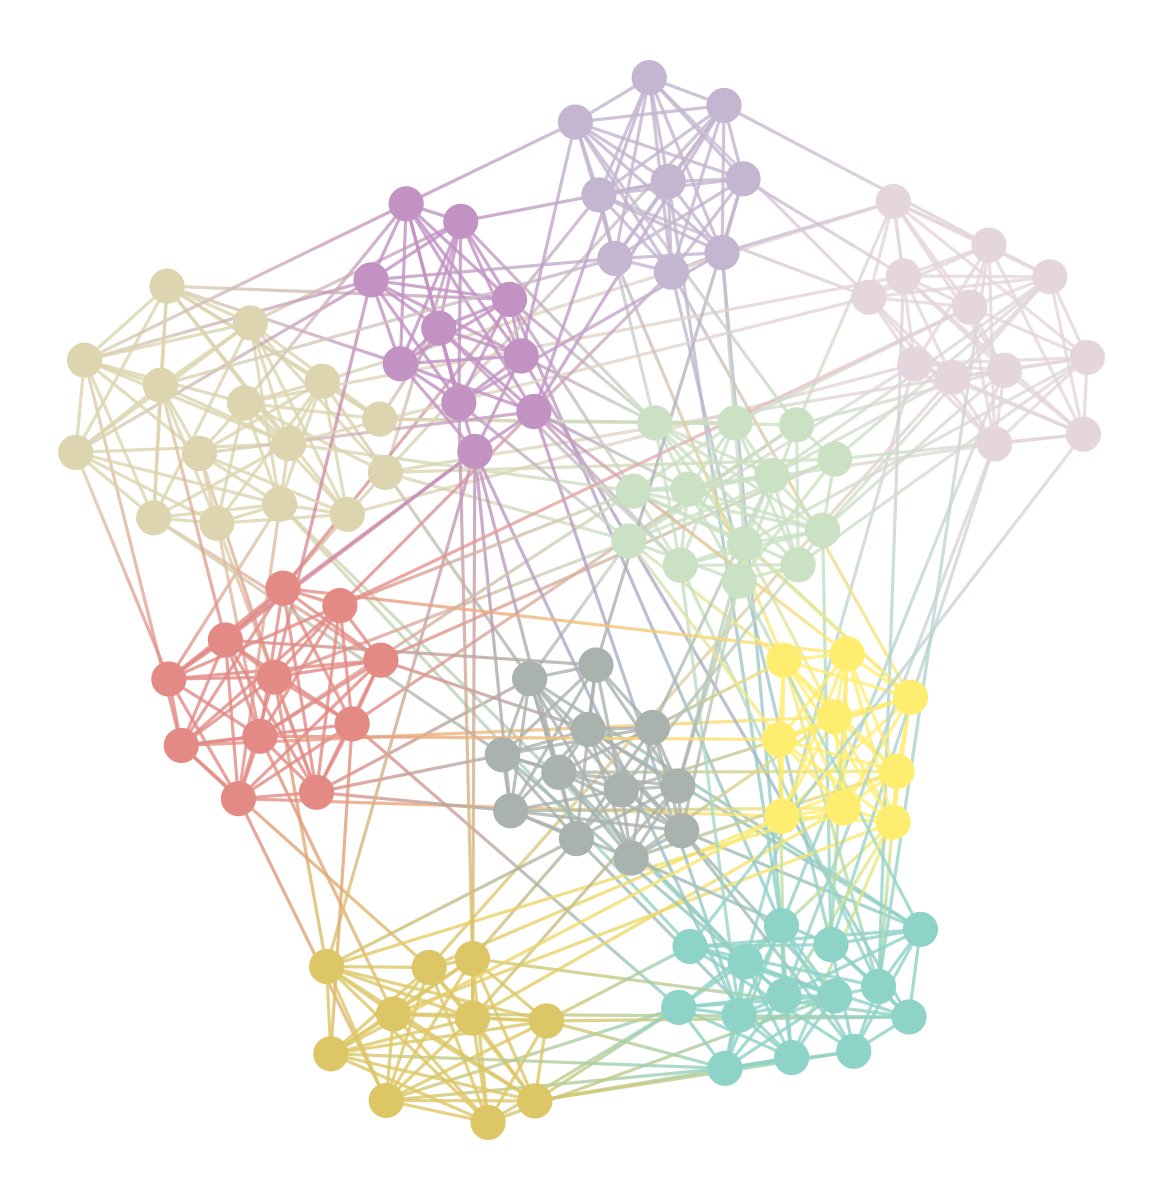
\includegraphics[width=\textwidth]{./assortative.png}
        \column{0.55\textwidth}
        \underline{Degree-corrected stochastic blockmodels}
        \begin{align*}
            \pi      & = [\pi_1, \pi_2, ..., \pi_d]  \\
            Z_i      & \diid \text{Categorical}(\pi) \\
            \theta_i & \diid F_\theta                \\
            B        & = 
            \begin{bmatrix}
                B_{11} & B_{12} & \dots  & B_{1d} \\
                B_{21} & B_{22} & \dots  & B_{2d} \\
                \vdots & \vdots & \ddots & \vdots \\
                B_{d1} & B_{d2} & \dots  & B_{dd} \\
            \end{bmatrix} \in [0, 1]^{d \times d}
        \end{align*}
        \begin{equation*}
            \P[\Z, \theta]{A_{ij} = 1} = \theta_i Z_i B Z_j^T \theta_j
        \end{equation*}
    \end{columns}
\end{frame}

\begin{frame}{We investigate identification when treatments depend on network structure}
    \begin{columns}
        \column{0.45\textwidth}
        \centering
        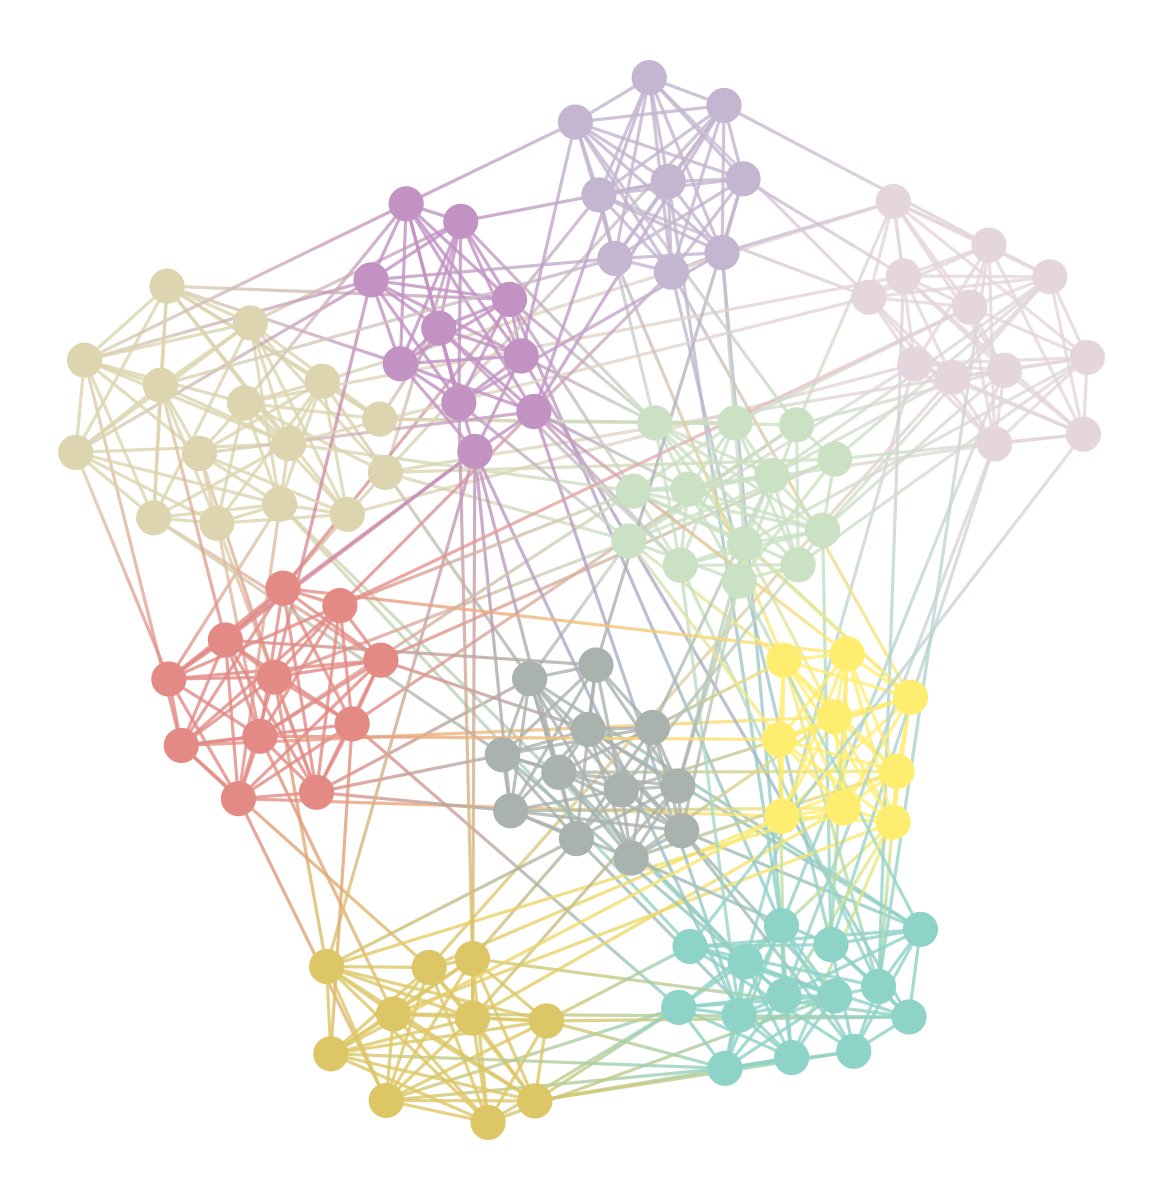
\includegraphics[width=\textwidth]{./assortative.png}
        \column{0.55\textwidth}
        \vspace{1mm}
        \begin{equation*}
            Z_i = \begin{bmatrix}
                0 & 1 & 0 & 0
            \end{bmatrix}
            ~\text{ and }~
            Z_j = \begin{bmatrix}
                0 & 0 & 1 & 0
            \end{bmatrix}
        \end{equation*}
        \begin{align*}
             & \P[Z, \theta]{A_{ij} = 1}                                      \\
             & \quad =
            \theta_i 
            \begin{bmatrix}
                0 \\
                1 \\
                0 \\
                0 
            \end{bmatrix}^T
            \begin{bmatrix}
                B_{11}                  & B_{1 \leftrightarrow 2} & B_{1 \leftrightarrow 3} & B_{1 \leftrightarrow 4} \\
                B_{1 \leftrightarrow 2} & B_{22}                  & B_{2 \leftrightarrow 3} & B_{2 \leftrightarrow 4} \\
                B_{1 \leftrightarrow 3} & B_{2 \leftrightarrow 3} & B_{33}                  & B_{3 \leftrightarrow 4} \\
                B_{1 \leftrightarrow 4} & B_{2 \leftrightarrow 4} & B_{3 \leftrightarrow 4} & B_{44}                  \\
            \end{bmatrix}
            \begin{bmatrix}
                0 \\
                0 \\
                1 \\
                0 
            \end{bmatrix}
            \theta_j
            \\ 
             & \quad = \theta_i \cdot B_{2 \leftrightarrow 3} \cdot \theta_j
        \end{align*}
        Consider the $X_i$ in place of $T_i$ where
        \begin{equation*}
            X_i = \theta_i Z_i
        \end{equation*}
    \end{columns}
\end{frame}

\begin{frame}{Identification is possible when treatments depend on network structure}
    \begin{theorem}
        Suppose that $A$ is sampled from a degree-corrected stochastic blockmodel. Define $X_i = \theta_i Z_i$. Let 
        \begin{equation*}
            Y = \alpha 1_n + \beta G Y + X \gamma + G X \delta + \varepsilon
        \end{equation*}
        for $\alpha, \beta \in \R$ and $\gamma, \delta \in \R^d$. Suppose that $X$ has $k \ge 2d$ distinct rows. Then, under some conditions,
        \begin{equation*}
            W_n = \begin{bmatrix}
                1_n & GY & X & GX
            \end{bmatrix}
        \end{equation*}
        converges uniformly to a limit object with rank $2d$ out of $2d + 2$. If any two entries of $(\alpha, \beta, \delta_1, ..., \delta_d)$ are set to zero in the data generating process, the limit object of $W_n$ is a matrix with full rank.
    \end{theorem}
    \vspace{4mm}
    \footnotesize * We aren't recommending this model, merely demonstrating that identification is feasible via dependence between the network and nodal covariates
\end{frame}

% \begin{frame}
%     \underline{Scaling by $\theta_i$}: Must scale by $\theta_i$ \\
%     \vspace{5mm}
%     \underline{$X$ latent}: but estimable via principal components analysis \citep{athreya2018}
% \end{frame}


% \begin{frame}{We performed a simulation study to confirm the theoretical results}
%     \begin{columns}
%         \begin{column}{0.5\textwidth}
%             \centering
%             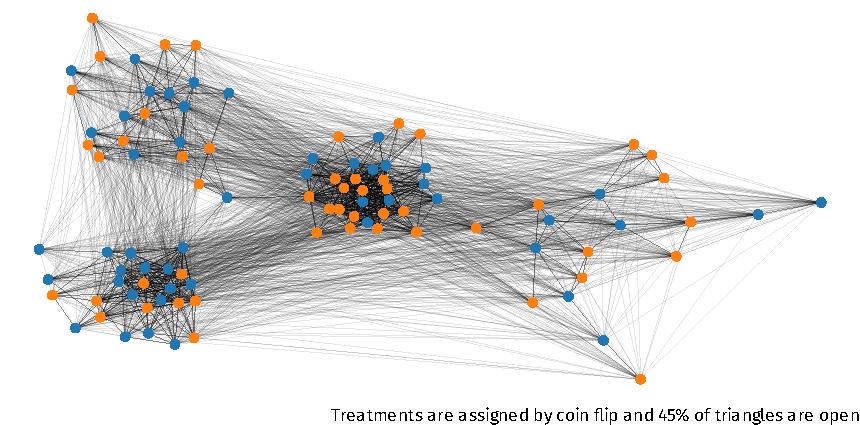
\includegraphics[width=\textwidth]{./figures/simulations/defense-backbone.pdf}
%         \end{column}
%         \begin{column}{0.5\textwidth}
%             \centering
%             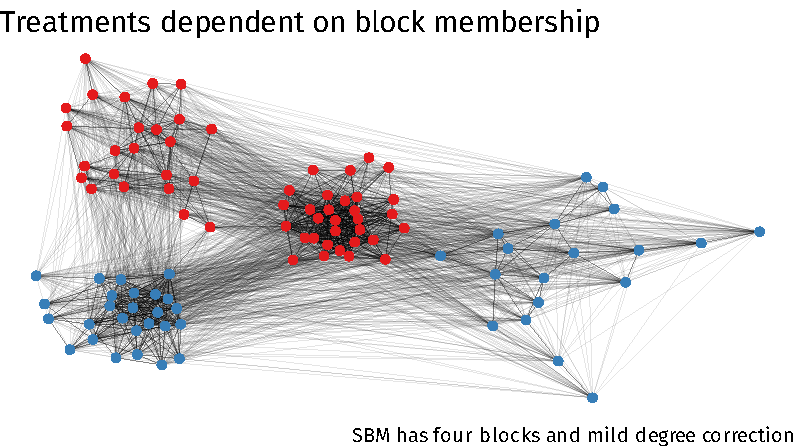
\includegraphics[width=\textwidth]{./figures/simulations/defense-backbone-dependent.pdf}
%         \end{column}
%     \end{columns}
% \end{frame}

\begin{frame}{We performed a simulation study to confirm the theoretical results}
    Sample network from degree-corrected stochastic blockmodel with $n$ nodes
    \begin{align*}
        \pi      & = [1/4, 1/4, 1/4, 1/4]                        \\
        \theta_i & \diid \mathrm{Uniform}[1, 2]                  \\
        B        & =
        \begin{bmatrix}
            0.5 & 0.1 & 0.1 & 0.1 \\
            0.1 & 0.5 & 0.1 & 0.1 \\
            0.1 & 0.1 & 0.5 & 0.1 \\
            0.1 & 0.1 & 0.1 & 0.5 \\
        \end{bmatrix}                                 \\
        n        & \in \set{100, 163, 264, 430, 698, 1135, 1845}
    \end{align*}
    Scale $B$ such that $\E{d_i} = 2 n^{0.7}$
\end{frame}

\begin{frame}{The simulations considered asymptotically \textcolor{BrickRed}{unidentified} and identified models}
    \begin{itemize}
        \setlength\itemsep{1.75em}
        \item \textcolor{BrickRed}{RCT model}: Treatment random and independent of network. $T_i \diid \Bern(0.5)$
              \begin{equation*}
                  Y = \textcolor{BrickRed}{\alpha} 1_n + \textcolor{BrickRed}{\beta} G Y + T \gamma + G T \textcolor{BrickRed}{\delta} + \varepsilon,
              \end{equation*}
              with $\textcolor{BrickRed}{\alpha} = 3, \textcolor{BrickRed}{\beta} = 0.2, \gamma = 4, \textcolor{BrickRed}{\delta} = 2$ and $\varepsilon \diid \calN(0, \sigma^2)$ with $\sigma = 0.1$.
        \item \textcolor{BrickRed}{Unrestricted model}: Treatment random and dependent on network. Define $X_i = \theta_i Z_i \in \R^4$
              \begin{equation*}
                  Y = \textcolor{BrickRed}{\alpha} 1_n + \textcolor{BrickRed}{\beta} G Y + X \gamma + G X \textcolor{BrickRed}{\delta} + \varepsilon,
              \end{equation*}
              where $\textcolor{BrickRed}{\alpha} = 3, \textcolor{BrickRed}{\beta} = 0.2$ and $\varepsilon \diid \calN(0, \sigma^2)$ with $\sigma = 0.1$. Since $X_i \in \R^4$, $\gamma, \textcolor{BrickRed}{\delta} \in \R^4$ and we fix $\textcolor{BrickRed}{\delta} = (2, 2, 2, 2)$ and $\gamma = (1.5, 2.5, 3.5, 4.5)$.
        \item Restricted model: The \emph{Unrestricted} model, but $\delta = (0, 0, 2, 2)$.
    \end{itemize}
\end{frame}

\begin{frame}{\textcolor{BrickRed}{Asymptotically unidentified} coefficients cannot be estimated}
    \centering
    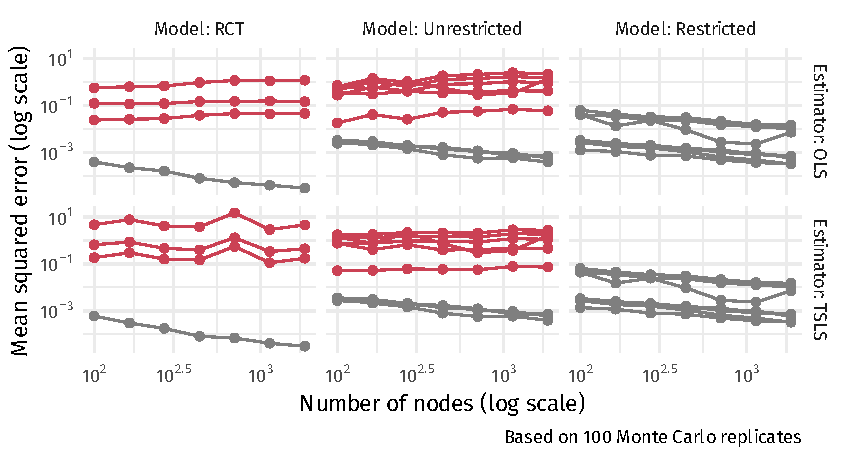
\includegraphics{./figures/simulations/defense-mse-all.pdf}
\end{frame}

\begin{frame}{We have important takeaways for social scientists}
    \begin{itemize}
        \item Linear-in-means models can be asymptotically unidentified
        \item Asymptotically unidentified peer effects cannot be estimated
        \item Treatments independent of network lead to identification failure
        \item Treatments dependent on network must considered on a case-by-case basis
    \end{itemize}
\end{frame}

\begin{frame}{Our work raises important methodological questions}
    \begin{itemize}
        \item Are there realistic models of network-treatment dependence?
        \item What happens in longitudinal models?
        \item What happens in sparse networks?
        \item Are peer effects hopeless?
        \item What alternatives are there to linear-in-means models?
    \end{itemize}
\end{frame}

\begin{frame}{Thank you! Questions?}
    \begin{columns}
        \begin{column}{0.4\textwidth}
            \begin{itemize}
                \item[] \faIcon{twitter} \href{https://twitter.com/alexpghayes}{@alexpghayes}
                \item[] \faIcon[regular]{envelope} \href{mailto:alex.hayes@wisc.edu}{alex.hayes@wisc.edu}
                \item[] \faIcon{wordpress} \href{https://www.alexpghayes.com}{alexpghayes.com}
                \item[] \faIcon{github} \href{https://github.com/alexpghayes}{github.com/alexpghayes}
            \end{itemize}
        \end{column}
        \begin{column}{0.6\textwidth}
            \centering
            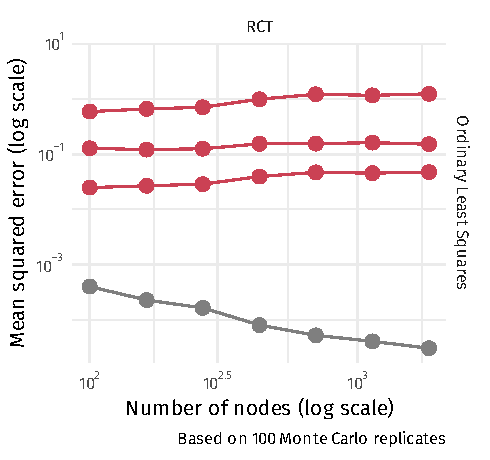
\includegraphics{./figures/simulations/defense-last-slide.pdf}
        \end{column}
    \end{columns}
\end{frame}

\appendix

\begin{frame}
    \underline{Estimators}
    \begin{itemize}
        \setlength\itemsep{1.25em}
        \item OLS: \texttt{lm($y \sim Gy + T + GT$)}
        \item TSLS: \texttt{ivreg($y \sim Gy + T + GT \mid T + GT + G^2T$)}
    \end{itemize}
\end{frame}

\begin{frame}
    \begin{proposition}[\citealt{bramoulle2009}]
        Suppose $\gamma \beta + \delta \neq 0$ (i.e., the peer effects are not zero). If $I, G$ and $G^2$ are linearly independent, in the sense that $a I + b G + c G^2 = 0$ requires $a = b = c = 0$, then $\alpha, \beta, \gamma$ and $\delta$ are identified.
    \end{proposition}
\end{frame}

\begin{frame}

    \begin{definition}[Random Dot Product Graph, \citealt{young2007}]
        Let $F$ be a distribution on $\R^d$ such that $0 \le x^T y$ for all $x,y \in \supp F$ and the convex cone of $\supp F$ is $d$-dimensional.
        Draw $X_1,X_2,\dots,X_n \diid F$, and collect these in the rows of $X \in \R^{n \times d}$ for ease of notation.
        Conditional on these $n$ vectors, which we call {\em latent positions}, generate edges by drawing the edges $\{ A_{ij} : 1 \le i < j \le n \}$ as independent $(\nu,b)$-subgamma random variables with $\bbE[ A_{ij} \mid X ] = \rho X_i^T X_j$, where $\rho \in [0,1]$.
        Then we say that $A$ is distributed according to an $n$-vertex random dot product graph with latent position distribution $F$, $(\nu,b)$-subgamma edges and sparsity factor $\rho$.
        We write $(A,X) \sim \RDPG( F, n)$, with the subgamma and sparsity parameters made clear from the context.
    \end{definition}
    
\end{frame}


\begin{frame}
    \begin{theorem}
        Suppose that $(A, X)$ are sampled from a random dot product model where $X$ is rank $d$ with probability $1$.
        Let $\varepsilon$ be a vector of mean zero, i.i.d.~$(\nu_\varepsilon, b_\varepsilon)$-subgamma random variables, with $(\nu_\varepsilon, b_\varepsilon)$ not depending on $n$,
        and let
        \begin{equation*}
            Y = \alpha 1_n + \beta G Y + X \gamma + G X \delta + \varepsilon
        \end{equation*}
        for $\alpha, \beta \in \R$ and $\gamma, \delta \in \R^d$. Suppose that $X$ has $k \ge 2d$ distinct rows. Then, under some conditions,
        \begin{equation*}
            W_n = \begin{bmatrix}
                1_n & GY & X & GX
            \end{bmatrix}
        \end{equation*}
        converges uniformly to a limit object with rank $2d$ out of $2d + 2$. If any two entries of $(\alpha, \beta, \delta_1, ..., \delta_d)$ are set to zero in the data generating process, the limit object of $W_n$ is a matrix with full rank, and $\alpha, \beta, \gamma, \delta$ are thus asymptotically identifiable.
    \end{theorem}
\end{frame}

\begin{frame}

    \begin{proposition}
        \label{prop:XHX-rank}
        Let $\mu = \E{X} \in \R^d$ and suppose that $Y_1,Y_2,\dots,Y_d,Z_1,Z_2,\dots,Z_d \in \R^d$ are rows of $X \in \R^{n \times d}$ such that $Y_1,Y_2,\dots,Y_d$ are linearly independent and $Z_1,Z_2,\dots,Z_d$ are linearly independent.
        \begin{equation*}
            H_Y = \diag\left( Y_1^T \mu, Y_2^T \mu, \dots, Y_d^T \mu \right)
            ~~~\text{ and }~~~
            H_Z = \diag\left( Z_1^T \mu, Z_2^T \mu, \dots, Z_d^T \mu \right).
        \end{equation*}
        Provided that $Z^{-1} H_Z^{-1} Z - Y^{-1} H_Y^{-1} Y \in \R^{d \times d}$ is invertible, then the matrix
        \begin{equation*} \label{eq:targetmx}
            M = \begin{bmatrix} X & H^{-1} X \end{bmatrix} \in \R^{n \times 2d}
        \end{equation*}
        has rank $2d$.
    \end{proposition}
    \underline{Morally:} need degree heterogeneity so that $X$ and $D^{-1} X$ are linearly independent
    % Also need to avoid knife-edge failure case where $F$ is funky
\end{frame}

\begin{frame}
    \begin{definition}[\citealt{boucheron2013}]
        Let $Z$ be a mean-zero random variable with cumulant generating function $\psi_Z(t) = \log \E{e^{t Z}}$.
        $Z$ is \emph{subgamma} with parameters $\nu \ge 0$ and $b \ge 0$ if
        \begin{equation*}
            \psi_Z(t) \le \frac{t^2 \nu}{2 (1 - b t)}
            ~\text{ and }~
            \psi_{-Z}(t) \le \frac{t^2 \nu}{2 (1 - b t)}
            ~\text{ for all }~ t < 1 / b.
        \end{equation*}
        We then write that $Z$ is $(\nu,b)$-subgamma.
    \end{definition}
    \vspace{4mm}
    \underline{Intuition}: tails decay at Gamma rates or faster \\
    \vspace{4mm}
    \underline{Examples}: Bernoulli, Poisson, Exponential, Gamma, Gaussian, sub-Gaussian, squared sub-Gaussians, bounded distributions, etc
\end{frame}

\begin{frame}
    \underline{Technical conditions for partial identification result} \\
    \vspace{6mm}
    \begin{itemize}
        \setlength{\itemsep}{1.75em}
        \item $\rho = \omega \left( \displaystyle \frac{ \log^2 n }{ \sqrt{n} } \right)$ and $\displaystyle \frac{ \nu + b^2 }{ \rho } = \Theta( 1 )$
        \item $\displaystyle \min_{i \in [n]} \abs*{X_i^T \, \E{X_1}} = \omega\left( \frac{ \log^2 n }{ \sqrt{ n } \rho } \right)$ almost surely.
        \item $\displaystyle \max_{i \in [n]} \| X_i \| = o(\sqrt{n})$ almost surely.
        \item $\displaystyle \bbE \| X_1 \|^2 < \infty$.
    \end{itemize}
\end{frame}

\bibliographystyle{chicago}
\bibliography{../references}

\end{document}